\chapter{Non-Inertial Frames; Dynamics on Earth}\label{ch:b1:non-inertial-frames}

Standing in a bus that turns left, you lean right, pushed by a force
nobody exerts. A bucket of water spun on a turntable hollows its surface
into a bowl. Under the dome of a museum a pendulum swings for hours,
and the line of its swing creeps slowly round, a few degrees an hour,
as if an invisible hand turned it. None of these is a new force: they
are what \omterm{thm:b1:newton-dynamics:laws}{Newton's laws} look like when the frame in which one describes
the motion is itself accelerating or rotating. This chapter shows how
velocities and accelerations transform between frames, how the laws of
dynamics are repaired by adding \emph{\omterm{thm:b1:non-inertial-frames:dynamics}{inertial forces}}, and what those
forces do on the most important rotating frame of all --- the Earth.

\begin{omfigure}
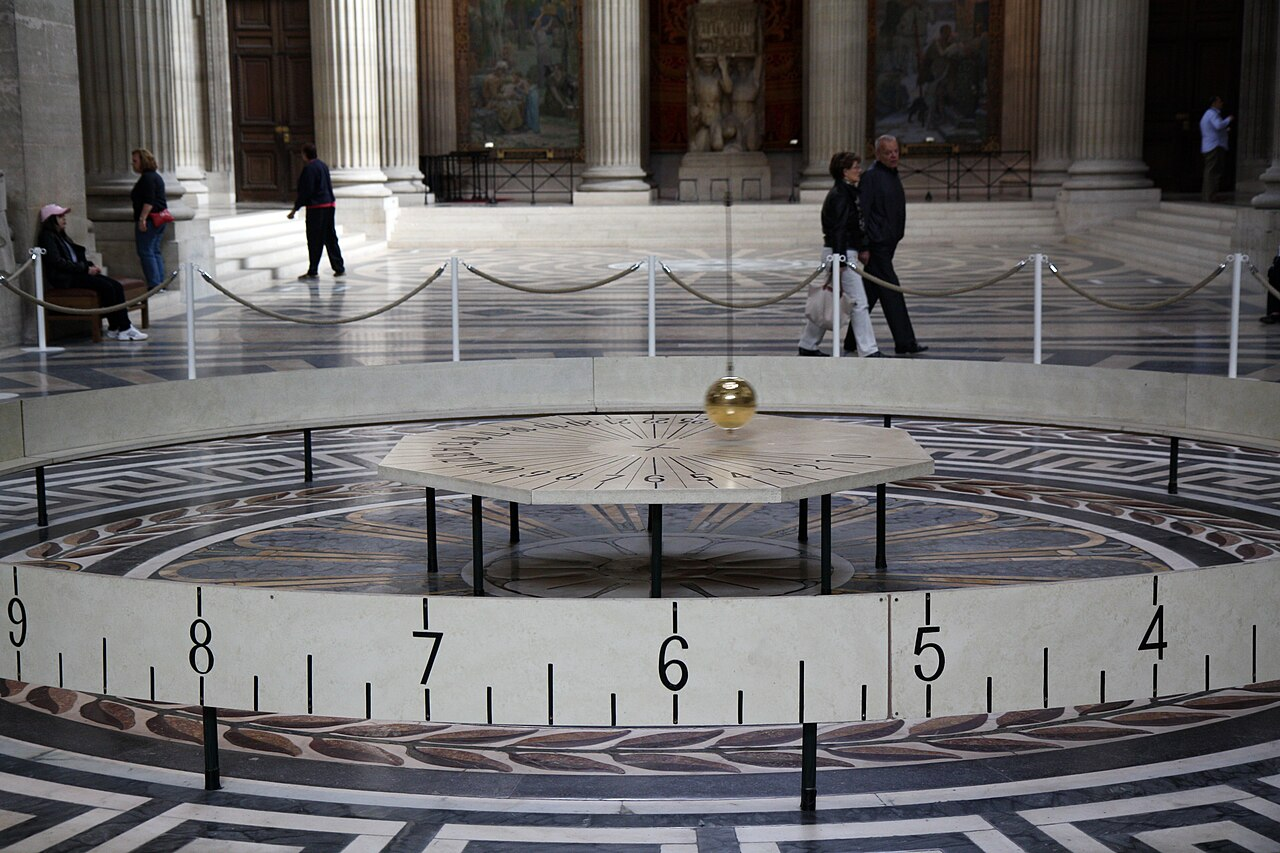
\includegraphics[width=0.55\linewidth]{images/book3/foucault-pendulum-pantheon.jpg}

{\small The \omterm{prop:b1:non-inertial-frames:foucault}{Foucault pendulum} of the Panthéon in Paris, where it was first hung in 1851: \qty{67}{m} of wire, a \qty{28}{kg} bob, and a plane of swing that turns with respect to the floor. Photograph: Olga Khomitsevich, CC~BY~2.0.}
\end{omfigure}

\section{Changing frame: kinematics}

\begin{definition}[Relative motion; frame in translation, in rotation]\label{def:b1:non-inertial-frames:frames}
\index{relative motion}\index{frame in translation}\index{frame in rotation}
Let $\mathcal R$ be a frame (origin $O$) and $\mathcal R'$ another (origin
$O'$) moving with respect to it. $\mathcal R'$ is \emph{in translation} if
its axes keep fixed directions in $\mathcal R$ (every point of $\mathcal R'$
has the velocity of $O'$); it is \emph{in rotation about a fixed axis}
$\Delta$ if $\Delta$ is fixed in both frames and $\mathcal R'$ turns about
it at the \omterm{cor:b1:point-kinematics:circular}{angular velocity} $\Omega(t)$. The velocity and acceleration of
a point $M$ \emph{relative} to $\mathcal R'$, $\vect v'$ and $\vect a'$, are
those a stationary observer of $\mathcal R'$ measures.
\end{definition}

\begin{theorem}[Composition of velocities and accelerations]\label{thm:b1:non-inertial-frames:composition}
\index{entrainment velocity}\index{entrainment acceleration}\index{Coriolis acceleration}
\begin{itemize}
  \item $\mathcal R'$ in translation with velocity $\vect v_{O'}$ and
        acceleration $\vect a_{O'}$:
        \[
        \vect v = \vect v' + \vect v_{O'}, \qquad \vect a = \vect a' + \vect a_{O'} .
        \]
  \item $\mathcal R'$ rotating about the fixed axis $\Delta$ at $\Omega$ (vector
        $\vect\Omega = \Omega\vect e_z$ along the axis); $H$ the projection
        of $M$ on the axis:
        \[
        \vect v = \vect v' + \vect\Omega\wedge\vect{HM}, \qquad
        \vect a = \vect a' + \underbrace{\big(-\Omega^2\vect{HM} + \dot\Omega\,\vect e_z\wedge\vect{HM}\big)}_{\vect a_e}
        + \underbrace{2\vect\Omega\wedge\vect v'}_{\vect a_C} .
        \]
\end{itemize}
$\vect a_e$ is the \emph{\omterm{thm:b1:non-inertial-frames:composition}{entrainment acceleration}} (the acceleration of the
point of $\mathcal R'$ that coincides with $M$: centripetal toward the axis
for uniform rotation), $\vect a_C = 2\vect\Omega\wedge\vect v'$ the
\emph{\omterm{thm:b1:non-inertial-frames:composition}{Coriolis acceleration}}, present only when $M$ moves relative to the
rotating frame.
\end{theorem}

\begin{proof}
Translation: $\vect{OM} = \vect{OO'} + \vect{O'M}$ with the components of
$\vect{O'M}$ in the common basis; differentiate twice. Rotation: use
\omterm{def:b1:point-kinematics:cylindrical}{cylindrical coordinates} about $\Delta$ in $\mathcal R$, $(r, \theta, z)$, and
in $\mathcal R'$, $(r, \theta', z)$ with $\theta = \theta' + \int\Omega\,\dd t$.
Then \cref{thm:b1:point-kinematics:cylindrical} in $\mathcal R$ with
$\dot\theta = \dot\theta' + \Omega$:
$\vect v = \dot r\vect e_r + r(\dot\theta' + \Omega)\vect e_\theta + \dot z\vect e_z
= \vect v' + r\Omega\vect e_\theta$, and $r\Omega\vect e_\theta = \vect\Omega\wedge\vect{HM}$.
For the acceleration, $\ddot\theta = \ddot\theta' + \dot\Omega$:
$\vect a = [\ddot r - r(\dot\theta' + \Omega)^2]\vect e_r + [r(\ddot\theta' + \dot\Omega)
+ 2\dot r(\dot\theta' + \Omega)]\vect e_\theta + \ddot z\vect e_z$; expanding and
grouping, $\vect a = \vect a' - r\Omega^2\vect e_r + r\dot\Omega\vect e_\theta
+ 2\Omega(-r\dot\theta'\vect e_r + \dot r\vect e_\theta)$, and the last bracket is
$2\vect\Omega\wedge\vect v'$ since $\vect e_z\wedge\vect e_r = \vect e_\theta$,
$\vect e_z\wedge\vect e_\theta = -\vect e_r$.
\end{proof}

\begin{example}[Walking on a turntable]\label{ex:b1:non-inertial-frames:turntable}
\cref{exo:b1:point-kinematics:12} computed the acceleration of a person
walking radially at $u$ on a turntable rotating at $\Omega$: $-ut\Omega^2\vect e_r
+ 2u\Omega\vect e_\theta$. In the new language: relative acceleration zero,
entrainment $-r\Omega^2\vect e_r$, Coriolis $2\vect\Omega\wedge u\vect e_r = 2u\Omega\vect e_\theta$.
\end{example}

\section{Dynamics in a non-inertial frame: inertial forces}

\begin{theorem}[Newton's law in a non-inertial frame]\label{thm:b1:non-inertial-frames:dynamics}
\index{inertial force}\index{centrifugal force}\index{Coriolis force}
In a frame $\mathcal R'$ that is not inertial, the motion of a particle
obeys
\[
m\vect a' = \sum\vect F + \vect F_e + \vect F_C, \qquad
\vect F_e = -m\vect a_e, \qquad \vect F_C = -m\vect a_C = -2m\vect\Omega\wedge\vect v' :
\]
Newton's second law holds provided one adds to the real forces the
\emph{entrainment force} (for a uniformly rotating frame, the
\emph{\omterm{thm:b1:non-inertial-frames:dynamics}{centrifugal force}} $+m\Omega^2\vect{HM}$, directed away from the
axis; for a \omterm{def:b1:non-inertial-frames:frames}{frame in translation}, $-m\vect a_{O'}$) and the \emph{\omterm{thm:b1:non-inertial-frames:dynamics}{Coriolis
force}}. These \emph{\omterm{thm:b1:non-inertial-frames:dynamics}{inertial forces}} are not interactions: no body
exerts them, they have no reaction, and they vanish in an \omterm{thm:b1:newton-dynamics:laws}{inertial
frame}.
\end{theorem}

\begin{proof}
$m\vect a = \sum\vect F$ in the \omterm{thm:b1:newton-dynamics:laws}{inertial frame} $\mathcal R$; substitute
$\vect a = \vect a' + \vect a_e + \vect a_C$ and move the two terms to the
right.
\end{proof}

\begin{example}[The leaning passenger, the plumb bob]\label{ex:b1:non-inertial-frames:bus}
In a bus braking at $a = \qty{3.0}{m/s^2}$, a hanging strap feels, in
the bus frame, gravity plus a forward \omterm{thm:b1:non-inertial-frames:dynamics}{inertial force} $ma$: it hangs
along the \emph{apparent gravity} $\vect g' = \vect g - \vect a_{O'}$, tilted
forward by $\arctan(a/g) = 17^\circ$. A passenger who wants to stand
still must lean into that apparent vertical. In an elevator falling
freely, $\vect g' = \vect 0$: weightlessness, seen from inside.
\end{example}

\begin{omfigure}
\begin{tikzpicture}[font=\small, x=1cm, y=1cm]
  % bus frame accelerating to the right (a): plumb bob tilts backward? braking: a points backward (left), bob tilts forward (right)
  \draw[thick] (-2.6,2.2) -- (2.6,2.2); \fill[pattern=north east lines] (-2.6,2.2) rectangle (2.6,2.4);
  \fill (0,2.2) circle (1.2pt);
  \draw[dashed] (0,2.2) -- (0,-0.2);
  \coordinate (B) at ($(0,2.2)+(-73:2.2)$);
  \draw[thick] (0,2.2) -- (B); \fill[omDef] (B) circle (3pt);
  \draw[-Stealth, omThm, very thick] (B) -- ++(0,-1.2) node[below] {$m\vect g$};
  \draw[-Stealth, omProp, very thick] (B) -- ++(0.9,0) node[right] {$-m\vect a_{O'}$};
  \draw[-Stealth, omExo, very thick] (B) -- ++(107:1.6) node[pos=0.6, left, xshift=-2pt] {$\vect T$};
  \draw (0,1.4) arc (-90:-73:0.8); \node at (0.3,1.15) {$\alpha$};
  \draw[-Stealth, thick] (-0.2,3.0) -- (-1.6,3.0); \node[below, font=\footnotesize] at (-0.9,2.95) {$\vect a_{O'}$ (braking)};
  \draw[-Stealth, thick] (0.4,3.0) -- (1.8,3.0); \node[below, font=\footnotesize] at (1.1,2.95) {motion};
  \begin{scope}[xshift=7.4cm]
  \draw[-Stealth, thick] (0,-0.4) -- (0,3.2) node[above] {$\Delta$};
  \draw[omDef!40, dashed] (0,1.0) ellipse (2.2 and 0.5);
  \fill[omDef] (2.2,1.0) circle (2.5pt) node[below right] {$M$};
  \draw[-Stealth, omProp, very thick] (2.2,1.0) -- ++(1.3,0) node[right] {$m\Omega^2\vect{HM}$};
  \draw[-Stealth, omExo, very thick] (2.2,1.0) -- ++(0.3,-0.95) node[below] {$-2m\vect\Omega\wedge\vect v'$};
  \draw[-Stealth, omThm, thick] (2.2,1.0) -- ++(-0.6,0.75) node[above] {$\vect v'$};
  \draw[-Stealth, omDef] (0.6,2.9) arc (80:20:0.6) node[right] {$\Omega$};
  \end{scope}
\end{tikzpicture}

{\small \omterm{thm:b1:non-inertial-frames:dynamics}{Inertial forces}. Left: in a braking bus the plumb bob hangs
along the apparent gravity $\vect g - \vect a_{O'}$, tilted forward. Right:
in a frame rotating at $\Omega$, a particle feels a \omterm{thm:b1:non-inertial-frames:dynamics}{centrifugal force} away
from the axis and, if it moves, a \omterm{thm:b1:non-inertial-frames:dynamics}{Coriolis force} perpendicular to its
relative velocity.}
\end{omfigure}

\begin{example}[The spinning bucket]\label{ex:b1:non-inertial-frames:bucket}
Water in a bucket rotating at $\Omega$ about its vertical axis is at rest
in the rotating frame under gravity and the \omterm{thm:b1:non-inertial-frames:dynamics}{centrifugal force}: its free
surface is perpendicular to the apparent gravity $\vect g' = -g\vect e_z +
\Omega^2r\vect e_r$ (the surface of a fluid at rest is normal to the field,
\cref{ch:b1:fluid-statics}). Its slope is $\dd z/\dd r = \Omega^2r/g$, so
$z = \Omega^2r^2/2g$: a paraboloid. At \qty{10}{rad/s} the rim of a
\qty{10}{cm} bucket stands \qty{5}{cm} above the center --- the principle
of the liquid-mirror telescope, whose spinning mercury takes exactly
the parabolic shape a mirror needs.
\end{example}

\begin{method}[Working in a non-inertial frame]\label{met:b1:non-inertial-frames:method}
Choose the frame in which the question is simplest (the bus, the
turntable, the Earth); list the real forces; add $-m\vect a_e$ and, if the
body moves in the frame, $-2m\vect\Omega\wedge\vect v'$; then proceed as in
\cref{met:b1:newton-dynamics:method}. Check: \omterm{thm:b1:non-inertial-frames:dynamics}{inertial forces} never
appear in the energy balance as ``work done by someone'' --- the \omterm{thm:b1:non-inertial-frames:dynamics}{Coriolis
force}, perpendicular to $\vect v'$, does no work; the \omterm{thm:b1:non-inertial-frames:dynamics}{centrifugal force}
derives from the \omterm{def:b1:work-and-energy:conservative}{potential energy} $-\tfrac12 m\Omega^2r^2$ in a uniformly
rotating frame.
\end{method}

\section{The terrestrial frame}

\begin{definition}[Geocentric and terrestrial frames]\label{def:b1:non-inertial-frames:earth}
\index{geocentric frame}\index{terrestrial frame}
The \emph{geocentric frame} has its origin at the Earth's center and
axes pointing to fixed stars; it is inertial to an excellent
approximation for motions of a day or less (its own acceleration around
the Sun is only \qty{6e-3}{m/s^2}, and nearly uniform over the Earth).
The \emph{terrestrial frame}, attached to the ground, rotates with
respect to it about the polar axis at
\[
\Omega = \frac{2\pi}{\qty{86164}{s}} = \qty{7.29e-5}{rad/s} .
\]
\end{definition}

\begin{proposition}[Weight, and the variation of $g$]\label{prop:b1:non-inertial-frames:weight}
\index{weight!and Earth's rotation}
In the \omterm{def:b1:non-inertial-frames:earth}{terrestrial frame} a body at rest feels the gravitational
attraction $m\vect{\mathcal G}$ and the \omterm{thm:b1:non-inertial-frames:dynamics}{centrifugal force} $m\Omega^2\vect{HM}$; their
sum is what a balance measures and a plumb line shows: the \emph{weight}
$m\vect g = m\vect{\mathcal G} + m\Omega^2\vect{HM}$. The centrifugal term is largest
at the equator, $\Omega^2R = \qty{0.034}{m/s^2}$, $0.35\%$ of $g$; it
reduces $g$ from the poles to the equator and tilts the vertical away
from the Earth's center by up to $0.1^\circ$ at mid-latitudes.
\end{proposition}

\begin{proof}
Apply \cref{thm:b1:non-inertial-frames:dynamics} with $\vect v' = \vect 0$
(no \omterm{thm:b1:non-inertial-frames:dynamics}{Coriolis force}); $\Omega^2R = (7.29\times10^{-5})^2 \times 6.37\times10^6$.
The deviation angle follows from the triangle of $m\vect{\mathcal G}$ and the
\omterm{thm:b1:non-inertial-frames:dynamics}{centrifugal force} (\cref{exo:b1:non-inertial-frames:6}).
\end{proof}

\begin{proposition}[The Coriolis force on Earth]\label{prop:b1:non-inertial-frames:coriolis}
At latitude $\lambda$, a body moving horizontally at speed $v'$ feels a
horizontal \omterm{thm:b1:non-inertial-frames:dynamics}{Coriolis force} of magnitude
\[
F_C = 2m\Omega v'\sin\lambda ,
\]
directed to the \emph{right} of the motion in the northern hemisphere and
to the left in the southern one, whatever the direction of travel; a
body falling vertically is deflected \emph{eastward} by $2m\Omega v'\cos\lambda$.
\end{proposition}

\begin{proof}
Decompose $\vect\Omega = \Omega(\cos\lambda\,\vect e_N + \sin\lambda\,\vect e_z)$
(north and local vertical). For horizontal $\vect v'$, $-2m\vect\Omega\wedge\vect v'$
has a horizontal part $-2m\Omega\sin\lambda\,\vect e_z\wedge\vect v'$ --- rotated
$90^\circ$ clockwise from $\vect v'$ seen from above, for $\lambda > 0$ ---
and a vertical part (negligible against gravity). For vertical $\vect v' =
-v'\vect e_z$: $-2m\Omega\cos\lambda\,\vect e_N\wedge(-v'\vect e_z) = 2m\Omega v'\cos\lambda\,
\vect e_E$, eastward.
\end{proof}

\begin{omfigure}
\begin{tikzpicture}[font=\small, x=1cm, y=1cm]
  \draw[omDef, thick] (0,0) circle (2.4);
  \draw[-Stealth, thick] (0,-3.0) -- (0,3.3) node[right] {$\vect\Omega$};
  \draw[dashed] (-2.6,0) -- (2.6,0);
  \coordinate (P) at (45:2.4);
  \fill[omThm] (P) circle (2pt);
  \draw[-Stealth, omThm, thick] (P) -- ++(45:1.0) node[right] {$\vect e_z$};
  \draw[-Stealth, omThm, thick] (P) -- ++(135:1.0) node[above left] {$\vect e_N$};
  \draw (0.9,0) arc (0:45:0.9); \node at (0.7,0.35) {$\lambda$};
  \draw[-Stealth, omExo, thick] (P) -- ++(45:0.45) ++(0,0) -- ++(0,0);
  \draw[-Stealth, omProp, very thick] (P) -- ++(0,1.2) node[above right] {$\vect\Omega$ (local)};
  \node[omProp, font=\footnotesize] at (3.0,1.2) {$\Omega\sin\lambda\,\vect e_z + \Omega\cos\lambda\,\vect e_N$};
  \begin{scope}[xshift=7.8cm]
  \draw[-Stealth] (-1.8,0) -- (2.0,0) node[right] {E};
  \draw[-Stealth] (0,-1.6) -- (0,2.0) node[above] {N};
  \draw[-Stealth, omThm, very thick] (0,0) -- (0,1.4) node[left] {$\vect v'$};
  \draw[-Stealth, omExo, very thick] (0,0.7) -- (1.1,0.7) node[right] {$\vect F_C$};
  \draw[omDef, thick, domain=0:1.5, samples=40] plot ({0.35*\x*\x},{\x});
  \node[font=\footnotesize] at (0.8,-0.9) {seen from above, $\lambda > 0$};
  \end{scope}
\end{tikzpicture}

{\small Left: at latitude $\lambda$ the Earth's rotation vector has a
vertical component $\Omega\sin\lambda$ and a northward one $\Omega\cos\lambda$.
Right: seen from above in the northern hemisphere, a body moving
horizontally is pushed to its right by the \omterm{thm:b1:non-inertial-frames:dynamics}{Coriolis force} and its path
curves clockwise.}
\end{omfigure}

\begin{example}[Small forces, big consequences]\label{ex:b1:non-inertial-frames:coriolisnum}
A train at \qty{100}{km/h} at latitude $45^\circ$: $a_C = 2 \times 7.29\times
10^{-5} \times 27.8 \times 0.71 = \qty{2.9e-3}{m/s^2}$, three thousandths of
$g$ --- the right-hand rail of a one-way track wears a little faster. Air
flowing at \qty{20}{m/s} toward a low-pressure center is turned right all
the way in and ends up circling it counterclockwise: every cyclone of the
northern hemisphere turns that way, every southern one the other. A stone
dropped down a \qty{100}{m} shaft at $45^\circ$ lands \qty{1.6}{cm} east of
the plumb line (\cref{exo:b1:non-inertial-frames:7}).
\end{example}

\begin{proposition}[Foucault's pendulum]\label{prop:b1:non-inertial-frames:foucault}
\index{Foucault pendulum}
A pendulum swinging with small \omterm{def:b1:wave-propagation:signal}{amplitude} at latitude $\lambda$ keeps its
plane of oscillation fixed with respect to the \omterm{def:b1:non-inertial-frames:earth}{geocentric frame}'s local
vertical rotation only: seen in the \omterm{def:b1:non-inertial-frames:earth}{terrestrial frame}, the plane turns
\emph{clockwise} (from above, northern hemisphere) at the angular rate
$\Omega\sin\lambda$, i.e.\ one full turn in
\[
T_F = \frac{\qty{23.93}{h}}{\sin\lambda} .
\]
\end{proposition}

\begin{proof}[Partial proof]
At the pole ($\lambda = 90^\circ$) the argument is geometric: no horizontal
force acts on the bob except the tension, whose horizontal component is
along the swing, so in the \omterm{def:b1:non-inertial-frames:earth}{geocentric frame} the plane of swing is fixed
while the Earth turns beneath it at $\Omega$; seen from the ground it turns
at $-\Omega$. At latitude $\lambda$, the horizontal \omterm{thm:b1:non-inertial-frames:dynamics}{Coriolis force} is
$-2m\Omega\sin\lambda\,\vect e_z\wedge\vect v'$: exactly what a frame rotating at
$\Omega\sin\lambda$ about the local vertical would produce. In a frame turning
with the plane at $-\Omega\sin\lambda$, that force disappears to first order
and the pendulum is an ordinary plane oscillator; hence the plane
precesses at $\Omega\sin\lambda$ in the \omterm{def:b1:non-inertial-frames:earth}{terrestrial frame}. The full
calculation, with the neglected second-order terms, is the weekend
problem.
\end{proof}

\begin{remark}[Tides, in two lines]\label{rem:b1:non-inertial-frames:tides}
\index{tides}
In the frame of the Earth's center, which falls freely toward the Moon,
the Moon's attraction is not uniform: a little stronger on the near side,
weaker on the far side. The difference, of order $2GM_{\text{Moon}}R/d^3
\approx \qty{1e-6}{m/s^2}$, stretches the oceans into two bulges --- two
tides a day --- and the Sun's contribution, $46\%$ of the Moon's, makes
spring and neap tides as the two align or cross
(\cref{exo:b1:non-inertial-frames:12}).
\end{remark}

\section{Exercises}

\begin{exercise}[$\star$]\label{exo:b1:non-inertial-frames:1}
A plumb bob hangs in a car accelerating at \qty{2.5}{m/s^2}: angle with
the vertical, and the tension in units of $mg$. Same car braking at the
same rate?
\end{exercise}

\begin{exercise}[$\star$]\label{exo:b1:non-inertial-frames:2}
A child sits \qty{3.0}{m} from the axis of a merry-go-round turning once
every \qty{4.0}{s}. Centrifugal acceleration in the rotating frame, as a
fraction of $g$; what real force provides it?
\end{exercise}

\begin{exercise}[$\star$]\label{exo:b1:non-inertial-frames:3}
Compute the Earth's \omterm{cor:b1:point-kinematics:circular}{angular velocity} $\Omega$, the centrifugal acceleration
at the equator, and its fraction of $g$. At what rotation period would
objects at the equator float off?
\end{exercise}

\begin{exercise}[$\star$]\label{exo:b1:non-inertial-frames:4}
A train of \qty{400}{t} runs at \qty{100}{km/h} at latitude $45^\circ$.
\omterm{thm:b1:non-inertial-frames:composition}{Coriolis acceleration} and the sideways force on the rails; which rail
is pushed, heading north? heading east?
\end{exercise}

\begin{exercise}[$\star\star$]\label{exo:b1:non-inertial-frames:5}
A bucket of radius \qty{10}{cm} spins at \qty{2.0}{rad/s}, then
\qty{10}{rad/s}. Rise of the water at the rim relative to the center.
Why is a spinning mercury bath a good telescope mirror?
\end{exercise}

\begin{exercise}[$\star\star$]\label{exo:b1:non-inertial-frames:6}
Show that the plumb line at latitude $\lambda$ deviates from the Earth's
center by about $\Omega^2R\sin\lambda\cos\lambda/g$ radians, and compute it
at $45^\circ$ in minutes of arc. By how much is $g$ smaller at the equator
than at the pole from rotation alone?
\end{exercise}

\begin{exercise}[$\star\star$]\label{exo:b1:non-inertial-frames:7}
A stone falls from rest down a \qty{100}{m} shaft at latitude $45^\circ$.
Treat the \omterm{thm:b1:non-inertial-frames:composition}{Coriolis acceleration} $2\Omega v\cos\lambda$ (eastward) as a small
perturbation with $v = gt$; integrate twice to find the eastward
deviation at the bottom. Why eastward?
\end{exercise}

\begin{exercise}[$\star\star$]\label{exo:b1:non-inertial-frames:8}
Precession period of a \omterm{prop:b1:non-inertial-frames:foucault}{Foucault pendulum} in Paris ($\lambda = 48.9^\circ$),
at the pole, and at the equator. Through what angle does the plane turn
in one hour in Paris?
\end{exercise}

\begin{exercise}[$\star\star$]\label{exo:b1:non-inertial-frames:9}
Air flows at \qty{20}{m/s} toward a low-pressure center at $45^\circ$
north. \omterm{thm:b1:non-inertial-frames:composition}{Coriolis acceleration}; in which sense does the air end up
circling the center? Why do small eddies (a sink, a tornado) not obey
this rule?
\end{exercise}

\begin{exercise}[$\star\star\star$]\label{exo:b1:non-inertial-frames:10}
A helium balloon on a string floats inside a car. When the car
accelerates forward, which way does the balloon lean? Explain with the
apparent gravity and buoyancy.
\end{exercise}

\begin{exercise}[$\star\star\star$]\label{exo:b1:non-inertial-frames:11}
A space station is a ring of radius \qty{100}{m} spun to give $1g$ of
artificial gravity at the rim. Rotation period? An astronaut walks along
the rim at \qty{1.5}{m/s}: \omterm{thm:b1:non-inertial-frames:composition}{Coriolis acceleration}, and its effect on his
apparent weight when walking with and against the rotation. He drops a
ball from \qty{2.0}{m}: roughly how far from his feet does it land?
\end{exercise}

\begin{exercise}[$\star\star\star$]\label{exo:b1:non-inertial-frames:12}
Show that the difference between the Moon's gravitational acceleration
at the Earth's center and at the point of the surface nearest the Moon is
about $2GM_Mr/d^3$ ($r$ the Earth's radius, $d$ the Earth--Moon distance);
compute it, and the same for the Sun; deduce the ratio of solar to lunar
tides.
\end{exercise}

\section{Problem: Foucault's pendulum}

\begin{problem}[{Weekend problem --- a 28-kilogram bob on a 67-meter
wire under a dome: why its plane of swing turns, how fast, what it
proves, and how small the force is that does it}]
\label{pb:b1:non-inertial-frames:1}
In 1851 a pendulum of length $\ell = \qty{67}{m}$ and mass $m = \qty{28}{kg}$
swung under the dome of the Panth\'eon in Paris, latitude $\lambda =
48.85^\circ$, with an \omterm{def:b1:wave-propagation:signal}{amplitude} of about $x_0 = \qty{3.0}{m}$. $\Omega =
\qty{7.29e-5}{rad/s}$, $g = \qty{9.81}{m/s^2}$.

\medskip
\noindent\textbf{Part I --- The pendulum as such.}
\begin{enumerate}
  \item Period of \omterm{prop:b1:work-and-energy:stability}{small oscillations}; check that the \omterm{def:b1:wave-propagation:signal}{amplitude} is small
        ($x_0/\ell$).
  \item Maximal speed of the bob, and its maximal height above the
        lowest point.
  \item Tension at the lowest point, in units of $mg$.
  \item Estimate the air drag on the bob at maximal speed (quadratic
        law, $C_xS \approx \qty{0.05}{m^2}$, $\rho = \qty{1.2}{kg/m^3}$) and
        compare with the maximal restoring force $m\omega_0^2x_0$.
  \item Why a long wire and a heavy bob? (Two reasons, one about the
        period, one about damping.)
\end{enumerate}

\medskip
\noindent\textbf{Part II --- At the pole.}
Imagine the same pendulum at the north pole.
\begin{enumerate}[resume]
  \item In the \omterm{def:b1:non-inertial-frames:earth}{geocentric frame}, list the forces on the bob and show
        that nothing can turn its plane of swing.
  \item Deduce what an observer standing on the ice sees the plane do,
        and in how long it returns to its initial direction.
  \item Describe the path of the bob on the ground (a rosette): how many
        petals in one day?
\end{enumerate}

\medskip
\noindent\textbf{Part III --- At latitude $\lambda$: the Coriolis term.}
Use local axes: $x$ east, $y$ north, $z$ up; \omterm{prop:b1:work-and-energy:stability}{small oscillations}, so the
motion is nearly horizontal, $\vect v' \approx (\dot x, \dot y, 0)$; the
restoring force is $-m\omega_0^2(x, y, 0)$ with $\omega_0 = \sqrt{g/\ell}$.
\begin{enumerate}[resume]
  \item Write $\vect\Omega$ in these axes.
  \item Compute $-2m\vect\Omega\wedge\vect v'$ and keep its horizontal
        components; show they involve only $\Omega\sin\lambda$.
  \item Write the two equations of motion for $x$ and $y$; set
        $\omega_F = \Omega\sin\lambda$ and compare $\omega_F$ with $\omega_0$.
  \item Introduce $u = x + jy$ and show that $\ddot u + 2j\omega_F\dot u +
        \omega_0^2u = 0$.
  \item Try $u = \eu^{j\alpha t}$: find the two values of $\alpha$, and
        show that for $\omega_F \ll \omega_0$ they are $\alpha \approx \pm\omega_0
        - \omega_F$.
  \item Deduce that $u \approx \eu^{-j\omega_Ft}(A\eu^{j\omega_0t} + B\eu^{-j\omega_0t})$:
        interpret the factor $\eu^{-j\omega_Ft}$ --- in which sense, at what
        rate, does the plane of swing turn?
  \item Compute the precession period in Paris and the angle turned in
        one hour.
  \item Why does the plane not turn at the equator?
\end{enumerate}

\medskip
\noindent\textbf{Part IV --- How small the force is.}
\begin{enumerate}[resume]
  \item Compute the maximal \omterm{thm:b1:non-inertial-frames:dynamics}{Coriolis force} on the bob and compare it
        with the weight and with the maximal restoring force.
  \item By how much is the swing's end point displaced sideways during
        one half-period? (The plane turns by $\omega_FT/2$.)
  \item In 1851 the bob carried a stylus that knocked over small pegs
        placed in a ring at the \omterm{def:b1:wave-propagation:signal}{amplitude}: about how long before the
        next peg fell?
  \item The pendulum was launched by burning a thread that held the bob
        aside. Why not push it by hand?
  \item Air drag stops a pendulum after a few hours. Modern museum
        pendulums use a small electromagnet at the bottom to restore
        energy without touching the plane of swing: why must that kick be
        strictly radial?
\end{enumerate}

\medskip
\noindent\textbf{Part V --- What it proves, and what else it does.}
\begin{enumerate}[resume]
  \item Foucault's demonstration convinced the public of the Earth's
        rotation. What exactly does the precession rate measure, and
        could the experiment determine the latitude?
  \item At which latitude would the plane turn once in exactly \qty{48}{h}?
  \item A gyroscope (a fast-spinning wheel in gimbals) keeps its axis
        fixed in the \omterm{def:b1:non-inertial-frames:earth}{geocentric frame}. Explain in one sentence why it too
        reveals the rotation, and name an application.
  \item Summarize: the one \omterm{thm:b1:non-inertial-frames:dynamics}{inertial force} responsible, its dependence on
        latitude, and the period it gives in Paris.
\end{enumerate}
\end{problem}
